% !TEX root = mainthesis.tex
%Chapter 6




\newcommand{\rb}{$^{87}$Rb\xspace}
\newcommand{\xyz}{$\ket{x,y,z}$\xspace}
\newcommand{\XYZ}{$\ket{X,Y,Z}$\xspace}

% Commands for bra-ket notation
\newcommand{\bra}[1]{\langle #1\vert}
\newcommand{\ket}[1]{\vert#1\rangle}
\newcommand{\braket}[2]{\langle #1\vert#2\rangle}

\newcommand{\reffig}[1]{Fig.~\ref{#1}}
\newcommand{\refeq}[1]{Eq.~(\ref{#1})}

\renewcommand{\thechapter}{6}

\chapter{Synthetic clock states}


Decoherence of quantum systems due to uncontrolled fluctuations of the environment presents fundamental obstacles in quantum science.
`Clock' transitions which are insensitive to such fluctuations are used to improve coherence, however, they are not present in all systems or for arbitrary system parameters.
Here, we create a trio of synthetic clock transitions
using continuous dynamical decoupling in a spin-1 Bose-Einstein condensate in which we observe a reduction of sensitivity to magnetic field noise of up to four orders of magnitude; this work complements the parallel work by Anderson et al.~(submitted, 2017).
In addition, using a concatenated scheme, we demonstrate suppression of sensitivity to fluctuations in our control fields.
These field-insensitive states represent an ideal foundation for the next generation of cold atom experiments focused on fragile many-body phases relevant to quantum magnetism, artificial gauge fields, and topological matter.

The loss of coherence due to uncontrolled coupling to a fluctuating environment is a limiting performance factor for quantum technologies~\cite{chaudhry_decoherence_2012,myatt_decoherence_2000,schlosshauer_decoherence_2005,viola_dynamical_1998}.
In select cases, first-order insensitive transitions --- `clock' transitions --- can mitigate the deleterious effect of the dominant noise sources, yet in most cases such transitions are absent~\cite{[{Quality oscillators that show remarkably precise and robust dynamics can be found even in biological systems. See for example the repressilator gene, }] potvin-trottier_synchronous_2016}.
Remarkably, under almost all circumstances, clock transitions can be synthesized using dynamical decoupling protocols.
These protocols involve driving the system with an external oscillatory field, resulting in a dynamically protected `dressed' system.

A number of dynamical decoupling protocols, pulsed or continuous, have been shown to isolate quantum systems from low-frequency environmental noise~\cite{cohen_continuous_2017,fanchini_continuously_2007,aharon_fully_2016,biercuk_optimized_2009,cai_robust_2012,bermudez_robust_2012,baumgart_ultrasensitive_2016,kazakov_magic_2015,sarkany_controlling_2014}.
Continuous dynamical decoupling (CDD) relies on the application of time-periodic continuous control fields, rather than a series of quantum-logic pulses.
Unlike conventional dynamical decoupling, CDD does not require any encoding overhead or quantum feedback measurements.

Thus far, CDD has inoculated multi-level systems in nitrogen vacancy centers in diamond, nuclear magnetic resonance experiments, and trapped atomic ions~\cite{laucht_dressed_2017,farfurnik_experimental_2017,noguchi_generation_2012,golter_protecting_2014,timoney_quantum_2011,webster_simple_2013,barfuss_strong_2015,rohr_synchronizing_2014}, from spatiotemporal magnetic field fluctuations.
We demonstrate CDD in atomic Bose-Einstein condensates (BECs) producing a protected three-level system of dressed-states, whose Hamiltonian is fully controllable.
The CDD-protected states are sensitive to fluctuations of the amplitude of the control field, and we  demonstrate that a second coupling field protects against those in a concatenated manner~\cite{cohen_continuous_2017,farfurnik_experimental_2017,cai_robust_2012}.
\begin{figure}[t]
    \centering
    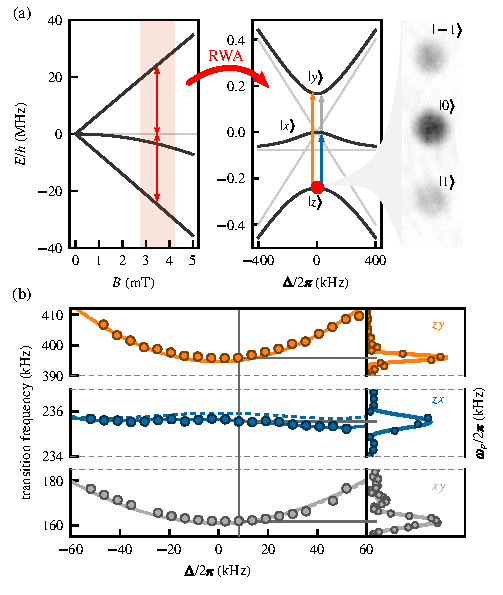
\includegraphics[]{Figures/Chapter6/fig1.pdf}
    \caption{(a) Left: dependence of the $5^2S_{1/2}$, $F=1$ ground state of \rb on magnetic field, where the quadratic dependence of the $\ket{m_F=0}$ state's Zeeman shift has been exaggerated so it is visible on the same scale.
    Center: energies of the \xyz eigenstates, for $\Omega/2\pi=\SI{200}{kHz}$ (black curves) and $\Omega=0$ (grey curves).
    Right: TOF image of $\ket{z}$ at $\Delta=0$, showing the constituent $m_F$ states.
    (b) Left: spectroscopic data showing transitions between the \xyz states for $\Omega/2\pi = \SI{194.5(1)}{kHz}$.
    The vertical scale of the center panel ($zx$ transition) has only 10\% the range of the other panels.
    The dashed lines correspond to the Hamiltonian of 
   while the solid lines include the dependence of the quadratic shift on $\Delta$.
    Right: representative spectra.}
    \label{fig:1}
\end{figure}

% \begin{figure}[t]
%     \centering
%     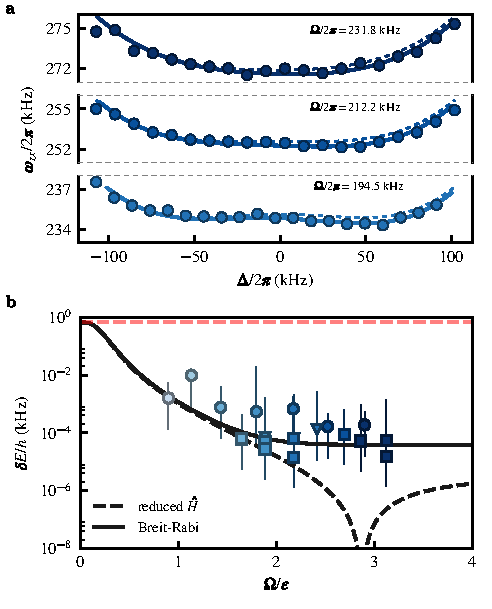
\includegraphics[]{Figures/Chapter6/fig2.pdf}
%     \caption{(a) Transition frequency $\omega_{zx}/2\pi$ for three values of $\Omega/2\pi$.
%     The dashed curves correspond to \refeq{eq:h}, while the solid curves use the Breit-Rabi expression.
%     (b) The change in energy from our experimental detuning fluctuations as measured in the $m_F$ basis is $\delta \Delta/2\pi = \SI{0.67}{kHz}$ (red dashed line).
%     Triangles correspond to \xyz spectroscopy data, squares to side-of-peak $\pi$-pulse data, and circles to double-dressed data.
%     The black dashed (solid) curve was calculated using \refeq{eq:h} (the Breit-Rabi expression).
%     The shading of the data points corresponds to the Rabi frequencies in \reffig{fig:3}.}
%     \label{fig:2}
% \end{figure}

% \textit{System.}
% We implemented CDD using a strong radio-frequency (RF) magnetic field with strength $\Omega$, that linked the three $m_F$ states comprising the $F=1$ electronic ground state manifold of \rb.
% The RF field was linearly polarized along ${\bf e}_x$, and had angular frequency $\omega$ close to the Larmor frequency $\omega_0 = g_F \mu_{\rm B} B_0$ from a magnetic field $B_0 {\bf e}_z$; $g_F$ is the Lande $g$-factor and $\mu_{\rm B}$ is the Bohr magneton.
% We coupled the dressed states using a weaker probe field with strength $\Omega_p$, polarized along ${\bf e}_y$ with angular frequency $\omega+\omega_p$ (\reffig{fig:1}a).
% Using the rotating wave approximation (RWA) for the frame rotating at $\omega$ (valid when $\omega_0 \gg \Omega,\,\Omega_p,\,\omega_p$), the system is described by
% \begin{align}
%     \hat H = \Delta\hat F_z &+ \hbar\epsilon(\hat F_z^2 / \hbar^2 - \hat{\mathbb I}) + \Omega \hat F_x \nonumber \\
%     &+ \Omega_p \left(\sin(\omega_p t) \hat F_x + \cos(\omega_p t) \hat F_y\right),
%     \label{eq:h}
% \end{align}
% with detuning $\Delta=\omega-\omega_0$; quadratic Zeeman shift $\epsilon$; spin-1 angular momentum operators $\hat F_{x,y,z}$; and identity operator $\hat{\mathbb I}$.  For $\Omega_p = 0$ the resulting eigenstates, denoted by $\ket{x}$, $\ket{y}$, and $\ket{z}$, are linear combinations of $\ket{m_F=0,\pm1}$.
% The corresponding eigenvalues for $\Delta = 0$ are $\omega_x = 0$ and $\omega_{z,y} = -(\epsilon \pm \sqrt{4 \Omega^{2} + \epsilon^{2}})/2$.
% The energy differences $\hbar\omega_{xy}$, $\hbar\omega_{zy}$ and $\hbar\omega_{zx}$ are only quadratically sensitive to $\Delta$ for $\Delta\ll\Omega$~\footnote{The energies are quadratic in $\Delta$ for $\Delta\ll\Omega$, and linear for $\Delta\gg\Omega$ with a slope of \SI{7}{MHz/mT}.} so that detuning fluctuations $\delta \Delta$ are suppressed to first order, making these a trio of synthetic clock states.
% At an optimal $\Omega$, $\omega_{zx}$ depends quartically on $\Delta$~\cite{xu_coherence-protected_2012,rabl_strong_2009}.
% For $\Delta \gg \Omega$ the \xyz states adiabatically connect to the corresponding $\ket{m_F=1,0,-1}$, states (\reffig{fig:1}b).
% As $\Omega\rightarrow 0^+$ and for $\Delta=0$, the \xyz states continuously approach the \XYZ states familiar from quantum chemistry.
% In contrast, as $\Omega\to\infty$ they become eigenstates of the $\hat F_x$ operator: $\ket{y,x,z} \to \ket{m_x=+1,0,-1}$.
% Unlike for the $m_F$ basis, an oscillatory magnetic field can drive transitions between all pairs of the \xyz states with non-zero transition matrix elements (see Appendix~\ref{app:xyz} for more details).

% Our BECs had $N\approx\num{5e4}$ atoms, and were held in a crossed dipole trap with trapping frequencies $(f_x,\, f_y,\, f_z) = (42(3),\, 34(2),\, 133(3))$\,Hz~\footnote{All uncertainties herein represent the uncorrelated combination of statistical and systematic uncertainties.}.
% The $B_0 \approx \SI{3.27}{mT}$ bias field lifted the ground state degeneracy, giving an $\omega_0/2\pi = \SI{22.9}{MHz}$ Larmor frequency, with a quadratic shift $\epsilon/2\pi=\SI{76.4}{kHz}$.
% In our laboratory the ambient magnetic field fluctuations were dominated by contributions from line noise giving an rms uncertainty $\delta\Delta/2\pi = g_F \mu_{\rm B}\delta B/h=\SI{0.67(3)}{kHz}$.

% We used adiabatic rapid passage (ARP) to transfer atoms initially prepared in any of the $\ket{m_F = 0,-1,1}$ states into the corresponding \xyz states.  Beginning far from resonance ($\Delta(t=0)/2\pi \approx -\SI{450}{kHz}$) with all coupling fields off, we ramped on the RF dressing field in a two-step process. We first ramped from $\Omega=0$ to approximately half its final value in \SI{10}{ms}.
% By increasing the magnetic field $B_0$, we then ramped $\Delta$ to zero in \SI{12}{ms} using a non-linear ramp adiabatic with respect to the relevant energy gaps.
% After allowing $B_0$ to stabilize for \SI{30}{ms}, we ramped the RF dressing field to its final value $\Omega$ in \SI{10}{ms}, yielding the dynamically decoupled $\ket{y, x, z}$ states.

% We measured the population in the \xyz states, we adiabatically deloaded them back into the $m_F$ basis by ramping $B_0$ so that $\Delta$ approached its initial detuned value in \SI{2}{ms}, and then ramped off the dressing RF field in \SI{1}{ms}.
% We obtained the spin-resolved momentum distribution using standard time-of-flight (TOF) imaging techniques, with a  Stern-Gerlach field to spatially separate the spin components during TOF.
% The right panel of \reffig{fig:1}a shows such a TOF image for decomposition of $\ket z$ into the $m_F$ states in a typical TOF image.

% We confirmed our control and measurement techniques spectroscopically measuring the energy differences between the \xyz states with our prove field.
% Figure~\ref{fig:1}b shows the dependence of the $\omega_{xy}/2\pi$, $\omega_{yz}/2\pi$, and $\omega_{zx}/2\pi$ on detuning for $\Omega/2\pi=\SI{194.5(1)}{kHz}$ derived from spectra such as in the side panel with coupling strength $\Omega_p/2\pi \approx \SI{1}{kHz}$ and $\Delta/2\pi \approx \SI{9}{kHz}$.

% The dashed curves based on \refeq{eq:h} clearly depart from our measurements for the $zx$ transition.
% This departure results from neglecting the weak dependence of the quadratic shift $\epsilon$ on bias field $B_0$.  In near-perfect agreement with experiment, the solid curves from the full Breit-Rabi expression account for this dependency.

% \textit{Robustness.}
% The $zx$ transition is remarkably robust against magnetic field variations, as commonly result from temporal and spatial magnetic field noise in laboratory environments  (Fig. \reffig{fig:2}a).
% We focus on the $zx$ transition, which can be made virtually independent of magnetic field variations due to the similar curvature of $\omega_z(\Delta)$ and $\omega_x(\Delta)$ (see the middle panel of \reffig{fig:1}a).
% We quantified the sensitivity of this transition to field variations with three methods corresponding to the different markers in \reffig{fig:2}b.
% In each case we measured the energy shift from resonance as a function of detuning and then used a fourth order polynomial fit to extract the rms residuals $\delta \omega_{zx}$ due to the known detuning noise~\footnote{Our procedure also quantifies the small fluctuations that survive for spectra that are flat beyond second order, as in \refeq{eq:h}.}.
% (1) Triangles denote data using full spectroscopical measurements similar to \reffig{fig:2}a.
% (2) squares denote data in which a detuned $\pi$-pulse of the probe field transferred atoms from $\ket z$ to $\ket x$, a side-of-peak technique giving a signal first-order sensitive to changes in $\omega_{zx}$.
% (3) circles describe data using an adiabatic technique described below.
% The results are not consistent with the theory simple from \refeq{eq:h} (dashed) and instead require the Breit-Rabi expression (solid) to obtain full agreement~\footnote{The fluctuations can be even smaller for a given $\Omega$ if we allow for $\Delta \neq 0$ (see Supplemental Materials).}.

% Even at our smallest coupling $\Omega/2\pi=\SI{69(1)}{kHz}$ the typical magnetic field noise was attenuated by two orders of magnitude, rendering it essentally undetectable.
% Ideally, the radius of curvature of $\omega_{zx}(\Delta)$ changes sign at about $\Omega/2\pi = \SI{220}{kHz}$, leaving only a $\Delta^4$ contribution, however, in practice the small dependence of $\epsilon$ on $B$ prevents this perfect cancellation.
% \begin{figure}[t]
%     \centering
%     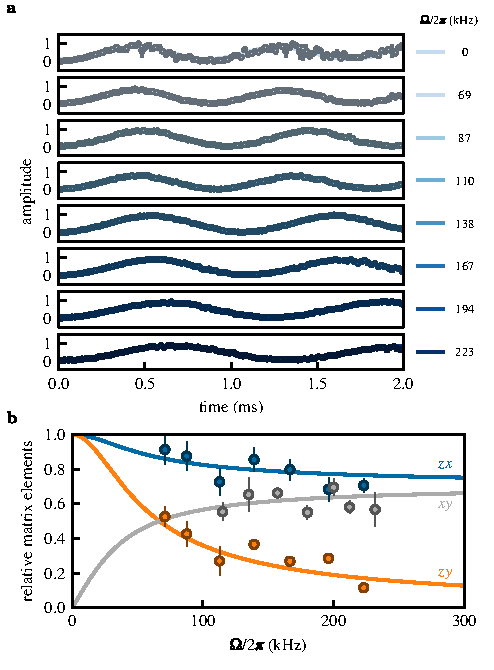
\includegraphics[]{Figures/Chapter6/fig3.pdf}
%     \caption{(a) Rabi oscillations.
%     Phase coherence is maintained throughout the oscillations in the dressed basis, while it is quickly lost in the $m_F$ basis.
%     The marker size reflects the typical uncertainties on the dressed basis oscillations.
%     (b) Transition matrix elements for $zx$ (blue) and $zy$ (orange) transitions decrease monotonically with increasing $\Omega$ for $\Delta=0$, while they increase for $xy$.
%     }
%     \label{fig:3}
% \end{figure}

% We explored the strength of the probe-driven transitions between these states by observing coherent Rabi oscillations (Fig. \reffig{fig:3}a) where our BEC was prepared in $\ket z$ and the probe field had strength $\Omega_p/2\pi\approx\SI{1}{kHz}$.
% The top panel shows Rabi oscillations between $\ket{m_F=0}$ and $\ket{m_F=-1}$ states for reference, and the remaining panels show oscillations between $\ket{z}$ and $\ket{x}$.
% The observed Rabi frequency between dressed states decreased with increasing $\Omega$ indicating a dependence of the $zx$ transition matrix elements on $\Omega$.
% These matrix elements, as well as those for the $zy$ transition, decrease with increasing $\Omega$ for $\Delta=0$ as shown in \reffig{fig:3}b and Appendix~\ref{app:me}.
% The coherence of the Rabi oscillations for longer times was limited by gradients in $\Omega$ that lead to phase separation of the dressed states, and therefore loss of contrast after a few tens of ms, but had no measurable effect on the coherence of the oscillations.
% In comparison, the coherence of the Rabi oscillation between the $m_F$ states deteriorates after \SI{500}{\us}.
% For these timescales, the loss of coherence was predominantly due to bias magnetic field temporal noise~\footnote{We cancelled gradient magnetic fields so that no phase separation of the bare states was observed for $>\SI{10}{sec}$.}.



% \textit{Concatenated CDD.}
% The driving field $\Omega$ coupled together the $\ket{m_F}$ states, giving us synthetic clock states \xyz that were nearly insensitive to magnetic field fluctuations.
% However, the spectrum of these states is first-order sensitive to fluctuations $\delta \Omega$ of the driving field.
% Reference~\cite{cai_robust_2012} showed that an additional field coupling together these \xyz states can produce doubly-dressed states that are insensitive to both $\delta \Omega$ and $\delta \Delta$: a process called concatenated CDD.
% In our experiment, the probe field provided the concatenating coupling field.
% Because $\Omega_p\ll\Omega$, we focus on a near-resonant two-level system formed by a single pair of dressed states, here $\ket{z}$ and $\ket{x}$, which we consider as pseudospins $\ket{\!\uparrow}$ and $\ket{\!\downarrow}$.
% These are described by the effective two-level Hamiltonian
% \begin{equation}
%     \hat H_p = \frac{\hbar\Delta'}{2} \hat \sigma_3 + \hbar\Omega' \cos(\omega_p t) \hat \sigma_1,
%     \label{eq:h2}
% \end{equation}
% with energy gap $\Delta' \approx \omega_{\downarrow, \uparrow}$ (shifted by off-resonant coupling to the $zy$ and $xy$ transitions) and coupling strength $\Omega' \propto \Omega_p$, as set by the matrix elements displayed in~\reffig{fig:3}b.
% Here $\hat \sigma_{1,2,3}$ are the three Pauli operators.
% \begin{figure}[t]
%     \centering
%     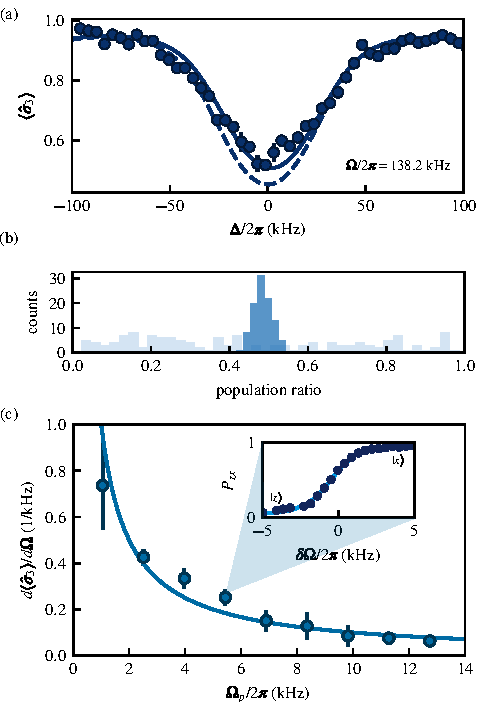
\includegraphics[]{Figures/Chapter6/fig4.pdf}
%     \caption{(a) The fractional population imbalance of the $\downarrow\uparrow$ transition for $\Omega/2\pi=\SI{138.2(1)}{kHz}$ over detuning $\Delta$.
%     The dashed curve is calculated using \refeq{eq:h} and the solid one using the full Breit-Rabi expression.
%     (b) The fidelity of preparing a balanced superposition of $\ket{\!\downarrow}$ and $\ket{\!\uparrow}$ (dark blue) states compared to $\ket{m_F=0}$ and $\ket{m_F=-1}$ states (light blue).
%     (c) The robustness of $\downarrow, \uparrow$ transition against fluctuations $\delta \Omega$ for different probe field coupling strengths.
%     The points represent the slope of the fitted curves to the fractional population imbalance (inset).}
%     \label{fig:4}
% \end{figure}
% A RWA of this Hamiltonian leads to the energy spectrum $E_{\uparrow,\downarrow} \approx \pm\Omega^\prime/2 + (\Delta^\prime)^2/2\Omega^\prime$, having again assumed the coupling $\Omega^\prime$ exceeds any fluctuations in $\Delta^\prime$.
% Thus, the concatenated CDD field protects from the fluctuations $\delta\Delta\prime$ of the first dressing field in the same way that CDD provided protection from detuning noise $\delta \Delta$.


% We produced doubly-dressed states by using the probe field near resonant with the $\downarrow, \uparrow$ transition and an ARP sequence.
% We started in $\ket{\!\downarrow}$ at $\Delta=0$ and ramped on the probe field $\Omega_p$ a few ms before ramping $\Omega$ to its final value.
% We chose  ARP parameters to create an equal superposition of $\ket{\!\downarrow}$ and $\ket{\!\uparrow}$ and quantified the sensitivity of this transition to large changes in the detuning in terms of the fractional population imbalance $\langle\hat\sigma_3\rangle = P_\downarrow(\Delta)-P_\uparrow(\Delta)$, shown in \reffig{fig:4}a for $\Omega/2\pi=\SI{138.2(1)}{kHz}$~\footnote{We chose the maximum value of $\Delta$ such that the population of \unexpanded{$\ket y$}, was negligible after deloading.}.
% This signal is first-order sensitive to $\omega_{\downarrow, \uparrow}$, and provided our third measurement of sensitivity to detuning in \reffig{fig:2}b denoted by circles.

% We compared the fidelity of preparing a superposition of the $\ket{\!\downarrow}$ and $\ket{\!\uparrow}$ states to adiabatically preparing a similar superposition of the the $\ket{m_F=0}$ and $\ket{m_F=-1}$ states, both with a probe field strength of  $\approx\SI{1}{kHz}$.
% Figure~\ref{fig:4}b shows the rms deviation of the population imbalance measured over a few hundred repetitions of the experiment.
% The rms deviation for the dressed basis is $0.024(1)$ and is and order of magnitude smaller than for the $m_F$ basis $0.29(1)$, where it practically impossible to prepare a balanced superposition for the parameters used here~\footnote{In \reffig{fig:4}b, the noise in the $m_F$ basis in not Gaussian distributed as is typical of line noise in these experiments.}.

% Figure~\ref{fig:4}c shows the response of the $\downarrow, \uparrow$ transition to small changes $\delta\Omega$ for different values of $\Omega_p$.
% We prepared an equal superposition of $\ket{\!\downarrow}$ and $\ket{\!\uparrow}$ following the same procedure as before for $\Omega/2\pi = \SI{138.2(1)}{kHz}$.
% We then measured how the population imbalance changes for small variations of $\Omega$ --- the effective detuning in the `twice-rotated frame' --- for different probe amplitudes $\Omega_p$.
% We defined a sensitivity parameter $d\langle\hat\sigma_3\rangle / d\Omega$, obtained from the linear regime of the population imbalance measurements (see inset in \reffig{fig:4}c).
% The robustness of the doubly-dressed states against $\delta \Omega$ fluctuations increased with $\Omega_p$, thus verifying the concatenating effect of CDD in the \xyz basis.

% \textit{Conclusions.}
% We realized a three-level system that is dynamically decoupled from low-frequency noise; measured now-allowed transitions between all three states; and demonstrated control techniques for creating arbitrary Hamiltonians.  These techniques add no heating or loss mechanisms, yet within the protected subspace retain the full complement of cold-atom coherent control tools such as optical lattices and Raman laser coupling, and permit new first-order transitions that are absent in the unprotected subspace.
% These transitions enable experiments requiring a fully connected geometry as for engineering exotic states, e.g., in cold-atom topological insulators, and two-dimensional Rashba spin-orbit coupling in ultracold atomic systems~\cite{campbell_rashba_2016, juzeliunas_generalized_2010}.

% The synthetic clock states form a decoherence-free subspace that can be used in quantum information tasks where conventional clock states might be absent, or incompatible with other technical requirements~\cite{bacon_universal_2000}.
% Moreover, their energy differences are proportional to the amplitude of the dressing field, and hence tunable, so they can be brought to resonance with a separate quantum system.
% The effective quantization axis can be arbitrarily rotated so that the two systems can be strongly coupled, pointing to applications in hybrid quantum systems~\cite{solano_chapter_2017,xiang_hybrid_2013}.
% Introducing a second coupling field shields the system from fluctuations of the first, a process which can be concatenated as needed.
% More broadly, synthetic clock states should prove generally useful in any situation where fluctuations of the coupling field can be made smaller than those of the environment.

\section{System}
\subsection{The xyz basis}
State decomposition, matrix elements, detuning dependence of energy something about resonantly coupling them

\section{Experiments}
\subsection{State preparation and deloading}
\subsection{Finding zero detuning}


\section{Robustness}

\section{Concatenated CCD}




